
%
\typeout{************************************************}
\typeout{Chapter 2 Prologue: Three Lessons Before We Begin}
\typeout{************************************************}
%
\begin{chapterptx}{Prologue: Three Lessons Before We Begin}{}{Prologue: Three Lessons Before We Begin}{}{}{x:chapter:Threelessons}
	%
	%
	\typeout{************************************************}
	\typeout{Section 2.1 Lesson One}
	\typeout{************************************************}
	%
	\begin{sectionptx}{Lesson One}{}{Lesson One}{}{}{x:section:ThreeLessons-lesson-one}
		Get a pad of paper and write down the answer to this question: What is .~.~.~No, really.  We're serious. \emph{Get a writing pad.} We'll wait.%
		\begin{aside}{}{g:aside:idp7}%
			We \emph{really} are serious about this. Get a pad of paper!%
		\end{aside}
		Got it? Good. Now write down your answer to this question: What is a number? Don't think about it. Don't analyze it. Don't consider it. Just write down the best answer you can without thinking. You are the only person who ever needs to see what you've written.%
		\par
		Done? Good.%
		\par
		Now consider this: All of the objects listed below are ``numbers'' in a sense we will not make explicit here. How many of them does your definition include?%
		\par
		%
		\begin{itemize}[label=\textbullet]
			\item{}\(\displaystyle 1\)%
			\item{}\(\displaystyle -1\)%
			\item{}\(\displaystyle 0\)%
			\item{}\(\displaystyle 3/5\)%
			\item{}\(\displaystyle \sqrt{2}\)%
			\item{}\(\displaystyle \sqrt{-1}\)%
			\item{}\(\displaystyle i^i\)%
			\item{}\(\displaystyle e^{5i}\)%
			\item{}\(4+3i-2j+6k\) (this is called a quaternion)%
			\item{}\(\dx{x}\) (this is the differential you learned all about in calculus)%
			\item{}\(\begin{pmatrix}
				1\amp 2\\-2\amp 1
			\end{pmatrix}\) (yes, matrices can be considered numbers).%
		\end{itemize}
		%
		\par
		Surely you included \(1\). Almost surely you included \(3/5\). But what about \(0?\) \(-1?\) Does your definition include \(\sqrt{2}?\) Do you consider \(\dx{x}\) a number? Leibniz\index{Leibniz, Gottfried Wilhelm} did. Any of the others? (And, yes, they really are all ``numbers.'')%
		\par
		The lesson in this little demonstration is this: You don't really have a clear notion of what we mean when we use the word ``number.'' And this is fine. Not knowing  is acceptable.%
		\begin{aside}{}{g:aside:idp8}%
			Sometimes it is even encouraged.%
		\end{aside}
		A principal goal of this  course of study is to rectify this, at least a little bit. When the course is over you may or may not be able to give a better definition of the word ``number'' but you will have a deeper understanding of the real numbers at least. That is enough for now.%
	\end{sectionptx}
	%
	%
	\typeout{************************************************}
	\typeout{Section 2.2 Lesson Two}
	\typeout{************************************************}
	%
	\begin{sectionptx}{Lesson Two}{}{Lesson Two}{}{}{x:section:ThreeLessons_lesson-two}
		Read and understand the following development of the Quadratic Formula.%
		\par
		Suppose \(a\neq0\). If%
		\begin{align}
			ax^2+bx+c =0\label{x:mrow:eq_QForm1}\\
			\intertext{then}
			x^2+\frac{b}{a}x\amp =-\frac{c}{a}\label{x:mrow:eq_QForm2}\\
			\intertext{Now let \(x=y-\frac{b}{2a}\) giving}
			y^2\amp = -\frac{c}{a} +\frac{b^2}{4a^2}\label{x:mrow:eq_QForm3}\\
			y\amp = \frac{\pm \sqrt{b^2-4ac}}{2a}\label{g:mrow:idp9}\\
			x\amp = \frac{-b\pm\sqrt{b^2-4ac}}{2a}\label{x:mrow:eq_QForm4}
		\end{align}
		%
		\par
		Were you able to follow the argument? Probably the step from \hyperref[x:mrow:eq_QForm1]{equation~({\xreffont\ref{x:mrow:eq_QForm1}})} to \hyperref[x:mrow:eq_QForm2]{equation~({\xreffont\ref{x:mrow:eq_QForm2}})} presented no difficulties. But what about the next step? Do you see where \hyperref[x:mrow:eq_QForm3]{equation~({\xreffont\ref{x:mrow:eq_QForm3}})} came from? If so, good for you. Most students, in fact most mathematicians, cannot make that step in their heads. But are you sure? Is there, perhaps, some small detail you've overlooked?%
		\par
		Check to see.%
		\par
		That is, let \(x=y-\frac{b}{2a}\) in \hyperref[x:mrow:eq_QForm2]{equation~({\xreffont\ref{x:mrow:eq_QForm2}})} and see if you can get \hyperref[x:mrow:eq_QForm3]{equation~({\xreffont\ref{x:mrow:eq_QForm3}})}. Do it on that handy pad of paper we told you to get out earlier. Do it now. We'll wait.%
		\begin{aside}{}{g:aside:idp10}%
			If you \emph{still} haven't gotten out a pad of paper, give up now. You're going to fail this course. Seriously. Do you think we would spend so much time on this, that we would repeat it so many times, if it weren't important. \emph{\emph{GET OUT A PAD OF PAPER NOW!}} Last chance. You've been warned.%
		\end{aside}
		Done? Good.%
		\par
		Perhaps you haven't been able to fill in the details on your own. That's ok. Many people can't. If not then get help: from a classmate, a friend, your instructor, whomever. Unfortunately most people won't get help in this situation. Instead they will perceive this as ``failure,'' hide it and berate themselves or the problem as ``stupid.'' In short they will let their personal insecurities and demons overwhelm them. \emph{Don't do this. Get help.} You are neither dumb nor incapable. There are a thousand reasons that on any given day you might not be able to solve this problem. But don't let a bad day interfere with the education you are here for. Get someone to help you over this hump. Later you will be able to help your helper in the same way. Really.%
		\par
		At this point we assume that you've successfully negotiated the transition from \hyperref[x:mrow:eq_QForm2]{equation~({\xreffont\ref{x:mrow:eq_QForm2}})} to \hyperref[x:mrow:eq_QForm4]{equation~({\xreffont\ref{x:mrow:eq_QForm4}})}.%
		\par
		See? It really wasn't that bad after all. Just a lot of elementary algebra. Now that you've done it (or seen it done), it is easy to see that there really wasn't much there.%
		\par
		But this is the point! We left those computations out precisely because we knew that they were routine and that you could fill in the details. Moreover, filling in the details yourself gives you a little better insight into the computations. If we'd filled them in for you we would have robbed you of that insight. And we would have made this book longer than it needs to be. We don't want to do either of those things. If we fill in all of the details of every computation for you, you won't learn to have confidence in your ability to do them yourself. And this book will easily double in length.%
		\par
		So the lesson here is this: Keep that pad of paper handy whenever you are reading this (or any other) mathematics text. You will need it. Routine computations will often be skipped. But calling them ``routine'' and skipping them does not mean that they are unimportant. If they were truly unimportant we would leave them out entirely.%
		\par
		Moreover ``routine'' does not mean ``obvious.'' Every step we took in the development of the Quadratic Formula was ``routine.'' But even routine computations need to be understood and the best way to understand them is to do them. This is the way to learn mathematics; it is the \emph{only} way that really works. Don't deprive yourself of your mathematics education by skipping the most important parts.%
		\begin{aside}{}{g:aside:idp11}%
			If you didn't fill in those details you're being stupid (or at least unduly stubborn). There is a good reason for putting these three lessons first. Stop wasting your time and intellect! Go do it now.%
		\end{aside}
		As you saw when you filled in the details of our development of the Quadratic Formula the substitution \(x=y-\frac{b}{2a}\) was crucial because it turned%
		\begin{equation*}
			x^2+\frac{b}{a}x +\frac{c}{a}=0
		\end{equation*}
		into%
		\begin{equation*}
			y^2=k
		\end{equation*}
		where \(k\) depends only on \(a\), \(b\), and \(c\). In the sixteenth century a similar technique was used by Ludovico Ferrari (1522-1565) to reduce the general cubic equation%
		\begin{equation}
			ax^3+bx^2+cx+d=0\label{x:men:eq_GenCubic}
		\end{equation}
		into the so-called ``depressed cubic''%
		\begin{equation*}
			y^3 +py+q=0
		\end{equation*}
		where \(p\), and \(q\) depend only on \(a\), \(b\), \(c\), and \(d\).%
		\par
		The general depressed cubic had previously been solved by Tartaglia (the Stutterer, 1500-1557) so converting the general cubic into a depressed cubic provided a path for Ferrari to compute the ``Cubic Formula'' \textemdash{} like the Quadratic Formula but better.%
		\begin{aside}{}{g:aside:idp12}%
			It is not entirely clear why eliminating the quadratic term should be depressing, but there it is.%
		\end{aside}
		\begin{figureptx}{\href{https://mathshistory.st-andrews.ac.uk/Biographies/Tartaglia/}{Tartaglia}\protect\footnotemark{}, ``The Stutterer''}{g:figure:idp13}{}%
			\begin{image}{0.36}{0.28}{0.36}%
				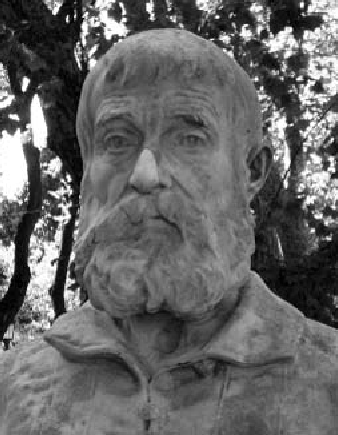
\includegraphics[width=\linewidth]{external/images/Tartaglia.png}
			\end{image}%
			\tcblower
		\end{figureptx}%
		\footnotetext[4]{\nolinkurl{mathshistory.st-andrews.ac.uk/Biographies/Tartaglia/}\label{g:fn:idp14}}%
		Ferrari also knew how to compute the general solution of the ``depressed quartic'' so when he and his teacher Girolomo Cardano (1501-1576) figured out how to depress a general quartic they had a complete solution of the general quartic as well. \begin{figureptx}{\href{https://mathshistory.st-andrews.ac.uk/Biographies/Cardan}{Girolomo Cardano}\protect\footnotemark{}}{g:figure:idp15}{}%
			\index{Cardano, Girolomo}\begin{image}{0.36}{0.28}{0.36}%
				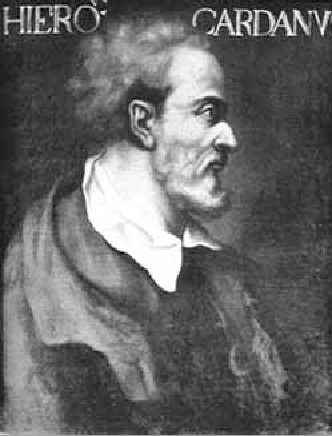
\includegraphics[width=\linewidth]{external/images/Cardan.png}
			\end{image}%
			\tcblower
		\end{figureptx}%
		\footnotetext[5]{\nolinkurl{mathshistory.st-andrews.ac.uk/Biographies/Cardan}\label{g:fn:idp16}}%
		Alas, their methods broke down entirely when they tried to solve the general quintic equation.  Unfortunately the rest of this story belongs in a course on Abstract Algebra, not Real Analysis.  But the lesson in this story applies to all of mathematics: Every problem solved is a new theorem which then becomes a tool for later use.  Depressing a cubic would have been utterly useless had not Tartaglia had a solution of the depressed cubic in hand.  The technique they used, with slight modifications, then allowed for a solution of the general quartic as well.%
		\par
		Keep this in mind as you proceed through this course and your mathematical education. Every problem you solve is really a theorem, a potential tool that you can use later. We have chosen the problems in this text deliberately with this in mind. Don't just solve the problems and move on. Just because you have solved a problem does not mean you should stop thinking about it. Keep thinking about the problems you've solved. Internalize them. Make the ideas your own so that when you need them later you will have them at hand to use.%
		\begin{problem}{}{g:problem:idp17}%
			%
			\begin{enumerate}[label=(\alph*)]
				\item{}Find \(M\) so that the substitution \(x=y-M\) depresses \hyperref[x:men:eq_GenCubic]{equation~({\xreffont\ref{x:men:eq_GenCubic}})}, the general cubic equation. Then find \(p\) and \(q\) in terms of \(a\), \(b\), \(c\), and \(d\).%
				\item{}Find \(K\) so that the substitution \(x=y-K\) depresses the general quartic equation. Make sure you demonstrate how you obtained that value or why it works (if you guessed it).%
				\item{}Find \(N\) so that the substitution \(x=y-N\) depresses a polynomial of degree \(n\). Ditto on showing that this value works or showing how you obtained it.%
			\end{enumerate}
			%
		\end{problem}
		\begin{problem}{Another Derivation of the Quadratic Formula.}{g:problem:idp18}%
			\index{Quadratic Formula!second proof} Here is yet another way to solve a quadratic equation. Read the development below with pencil and paper handy. Confirm all of the computations that are not completely transparent to you. Then use your notes to present the solution with \emph{all} steps filled in.%
			\begin{aside}{}{g:aside:idp19}%
				Be sure you are clear on the purpose of this problem before you begin. This is not about solving the Quadratic Equation. You already know how to do that. Our purpose here is to give you practice filling in the skipped details of mathematical exposition. We've chosen this particular problem because it should be a comfortable setting for you, but this particular solution is probably outside of your previous experience.%
			\end{aside}
			Suppose that \(r_1\) and \(r_2\) are solutions of \(ax^2+bx+c=0\). Without loss of generality suppose that \(a>0\).  Suppose further that \(r_1\ge r_2\).  Then%
			\begin{align*}
				ax^2+bx+c \amp = a(x-r_1)(x-r_2)\\
				\amp = a\left[x^2-(r_1+r_2)x+(r_1+r_2)^2-(r_1-r_2)^2-3r_1r_2\right]\text{.}
			\end{align*}
			%
			\par
			Therefore%
			\begin{align}
				r_1+r_2\amp = -\frac{b}{a}\label{x:mrow:eq_LagrangeQuadratic1}\\
				\intertext{and}
				r_1-r_2 \amp = \sqrt{\left(\frac{b}{a}\right)^2-\frac{4c}{a}}\text{.}\label{x:mrow:eq_LagrangeQuadratic2}
			\end{align}
			%
			\par
			Equations \hyperref[x:mrow:eq_LagrangeQuadratic1]{({\xreffont\ref{x:mrow:eq_LagrangeQuadratic1}})} and \hyperref[x:mrow:eq_LagrangeQuadratic2]{({\xreffont\ref{x:mrow:eq_LagrangeQuadratic2}})} can be solved simultaneously to yield%
			\begin{align*}
				r_1\amp =\frac{-b+\sqrt{b^2-4ac}}{2a}\\
				r_2\amp =\frac{-b-\sqrt{b^2-4ac}}{2a}\text{.}
			\end{align*}
			%
		\end{problem}
	\end{sectionptx}
	%
	%
	\typeout{************************************************}
	\typeout{Section 2.3 Lesson Three}
	\typeout{************************************************}
	%
	\begin{sectionptx}{Lesson Three}{}{Lesson Three}{}{}{x:section:ThreeLessons_lesson-three}
		In the hustle and bustle of a typical college semester, with a lot of demands on your time and very little time to think, it becomes very easy to see each problem you solve as a small, isolated victory and then move on to the next challenge. This is understandable. Each problem you solve \emph{is} a small victory and you've every right to be proud of it. But it is not isolated and it is a mistake to think that it is.%
		\begin{figureptx}{\href{https://mathshistory.st-andrews.ac.uk/Biographies/Polya/}{George Polya}\protect\footnotemark{}}{g:figure:idp20}{}%
			\begin{image}{0.36}{0.28}{0.36}%
				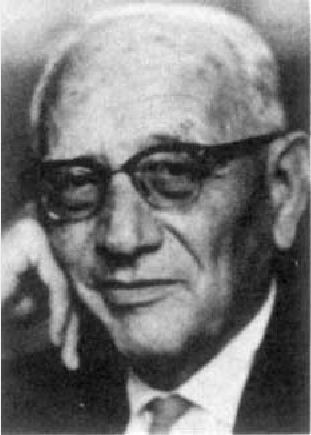
\includegraphics[width=\linewidth]{external/images/Polya.png}
			\end{image}%
			\tcblower
		\end{figureptx}%
		\footnotetext[6]{\nolinkurl{mathshistory.st-andrews.ac.uk/Biographies/Polya/}\label{g:fn:idp21}}%
		In his book \emph{How to Solve It} the mathematician and teacher George Polya gave four steps for problem solving. The steps may be paraphrased as%
		\begin{enumerate}
			\item{}Understand the problem.%
			\item{}Formulate a plan.%
			\item{}Execute the plan.%
			\item{}Reflect on what you've done.%
		\end{enumerate}
		%
		\par
		This process is iterative. That is, once a plan is formulated and executed we often find that our plan was not up to the task. So we have to ask what went wrong, form a new plan and try again. This is the fourth step: Reflect on what you've done.%
		\par
		Almost everyone remembers this fourth step when their plan \emph{doesn't} work. After all, you've got to try again so you have to ask what went wrong. But it is all too easy to neglect that crucial fourth step when the plan succeeds. In that case, flush with success we usually move on to the next problem and start over from scratch.%
		\par
		This is a mistake. Having solved a problem is no reason to stop thinking about it.%
		\par
		That fourth step is at least as important when we have succeeded as when we have failed. Each time you solve a problem stop and ask yourself a few questions:%
		\begin{itemize}[label=\textbullet]
			\item{}Are there any easy consequences that follow from the result?%
			\item{}How does it fit into the broader scheme of other problems you have solved?%
			\item{}How might it be used in the future?%
		\end{itemize}
		%
		\par
		Also, notice the structure of the problem. Some assumptions had to be made. What were they? Were they all necessary? That is, did your solution use everything that was assumed? If not, you may have something considerably more general than it at first appears. What is that more general statement? Even if you used all of the assumptions, was that really necessary? Can you solve a similar problem with weaker assumptions?%
		\par
		Take a moment to pack all of these questions (and their answers) away in your mind so that when you see something similar in the future you will be reminded of it. \emph{Don't} solve any problem and then forget it and move on. The nature of mathematics is cumulative. Remember, you are not here to accumulate grade points. You are here to learn and understand the concepts and methods of mathematics, to gain ``mathematical maturity.'' Part of that maturation process is the accumulation of a body of facts (theorems), and techniques that can be used to prove new theorems (solve new problems).%
		\par
		This text has been written with the maturation process in mind. You will frequently find that the problems you solve today can be used to good effect in the ones you attempt tomorrow, but only if you remember them. So take a moment after you've solved each problem to think about how it fits into the patterns you already know. This is important enough to bear repeating: \emph{A problem, once solved, becomes a tool for solving subsequent problems!}%
		\par
		The purpose of the following sequence of problems is to help you become accustomed to this notion (if you aren't already). It is a progression of results about prime numbers. As you probably recall, a prime number is any integer greater than \(1\) whose only factors are itself and \(1\). For example, \(2\), \(3\), \(5\), \(7\), \(11\) are prime, while \(4\), \(6\), \(9\) are not. A major result about prime numbers is the following:%
		\begin{theorem}{}{}{x:theorem:thm_FTA}%
			\alert{The Fundamental Theorem of Arithmetic}%
			\par
			Any integer greater than \(1\) is either prime or it is a product of prime numbers. Furthermore, this prime decomposition is unique up to the order of the factors.%
		\end{theorem}
		We will not prove this, but we will use it as a starting point to examine the following problems. As you do these problems, notice how subsequent problems make use of the previous results.%
		\par
		Notice that the notation \(p\,|a\) simply means that the integer \(p\) divides the integer \(a\) with no remainder.%
		\begin{problem}{Fermat's Little Theorem, step 1.}{g:problem:idp22}%
			\index{Fermat's Little Theorem!problems leading to!if a prime divides a product of two numbers then it divides one of the factors} Let \(p\) be a prime number and \(a, b\) positive integers such that \(p\, | (a\cdot b)\). Show that \(p\,|a\) or \(p\,|b\).%
			\par\smallskip%
			\noindent\textbf{\blocktitlefont Hint}.\hypertarget{g:hint:idp23}{}\quad{}If \(p\,|a\) then we are done. If not then notice that \(p\) is a prime factor of \(a\cdot b\). What does the Fundamental Theorem of Arithmetic say about the prime factors of \(a\cdot b\) compared to the prime factors of \(a\) and \(b?\)%
		\end{problem}
		\begin{problem}{Fermat's Little Theorem, step 2.}{g:problem:idp24}%
			\index{Fermat's Little Theorem!problems leading to!if a prime divides an arbitrary product then it divides one of the factors} Let \(p\) be a prime number and let \(a_1, a_2, \ldots,
			a_n\) be positive integers such that \(p\,|\left(a_1\cdot
			a_2\cdot a_3\cdot\ldots\cdot a_n\right)\).  Show that \(p\,|a_k\) for some \(k\in\{1, 2, 3, \ldots, n\}\).%
			\par\smallskip%
			\noindent\textbf{\blocktitlefont Hint}.\hypertarget{g:hint:idp25}{}\quad{}Use induction on \(n\) and the result of the previous problem.%
		\end{problem}
		\begin{problem}{Fermat's Little Theorem, step 3.}{g:problem:idp26}%
			\index{Fermat's Little Theorem!problems leading to!if \(p\) is prime then \(p\) divides \(p \choose{}k\)} Let \(p\) be a prime number and let \(k\) be an integer with \(1\le k\le p-1\). Prove that \(p\left|{p \choose{}k}\right.\), where \({p \choose{}k}\) is the binomial coefficient \(\frac{p!}{k!(p-k)!}\).%
			\par\smallskip%
			\noindent\textbf{\blocktitlefont Hint}.\({p\choose{}k}k!(p-k)!\).  How does the previous result apply?%
		\end{problem}
		We now have all the machinery in place to prove one of the really cool theorems from number theory.%
		\begin{theorem}{}{}{x:theorem:thm_FermatsLittleTheorem}%
			\alert{Fermat's Little Theorem}%
			\par
			\index{Fermat's Little Theorem} Let \(p\) be any prime number. Then \(p\,|(n^p-n)\) for all positive integers \(n\).%
		\end{theorem}
		\begin{problem}{Fermat's Little Theorem.}{g:problem:idp28}%
			\index{Fermat's Little Theorem} Prove Fermat's Little Theorem.%
			\par\smallskip%
			\noindent\textbf{\blocktitlefont Hint}.\hypertarget{g:hint:idp29}{}\quad{}Use induction on \(n\). To get from \(n\) to \(n+1\), use the binomial theorem on \((n+1)^p\).%
		\end{problem}
		Fermat's Little Theorem is the foundational basis for a number of results in number theory and encryption.%
	\end{sectionptx}
\end{chapterptx}
%
%